\chapter{Domain Driven Design}

\section{Ubiquitous Language (UL)}
\subsection*{Item}

\textbf{Bedeutung}: Ein \textit{Item} ist ein nicht-belebtes Objekt,
welches einen konkreten Gegendstand im Spiel wie etwa Waffen,
Rüstungen oder Münzen repräsentiert. Mit ihm kann interagiert werden.
Ein Item erfüllt verschiedene Funktionen abhängig vom Typ, wie etwa
Heilung, Stärkung des Spielers oder Beeinflussung des Spielstandes.

\textbf{Begründung}: Die Verwendung des Begriffes in der UL erlaubt
eine einheitliche Kommunikation zwischen den Entwicklern und Designern.
Hinzu kommt, dass der Begriff grundlegend in der Spieleentwicklung ist.
Somit lässt sich leichter festlegen, wie Items designed und logisch
in das Spielgeschehen integriert werden und wie diese die Spielerfahrung
formen.



\subsection*{Room}

\textbf{Bedeutung}: Der Begriff \textit{Room} definiert einen
abgegrenzten Bereich der Spielwelt. Jeder Raum stellt für den Spieler
eine neue Herausforderung dar. In ihm befinden sich neue Gegner und
neue Items. Besonders ersichtlich wird die Abgrenzung der Räume, wenn
sie abgeschlossen sind, weil in ihnen noch Gegner leben.

\textbf{Begründung}: Der Begriff Room in der UL ist essentiell wichtig,
da Entwickler und Designer sich absprechen müssen, um den technischen
und stilistischen Entwurf für abgegrenze Spielbereiche zu schaffen.
Für Entwickler ist der Begriff besonders prägend im Bereich der Welt-
Generierung. Für Designer ist er wichtig, um zwischen verschiedenen
Typen zu unterscheiden, welche unterschiedlich ausgebildet werden.



\subsection*{Level}

\textbf{Bedeutung}: Das \textit{Level} repräsentiert eine abgegrenzte
Spielstufe. Es gilt dieses komplett zu absolvieren, bis man den
End-Raum des Levels gefunden hat. Es stellt eine Einheit einzelner mit
einander verbundener Räume dar. Levels haben Fortschrittsmechanismen
bezogen auf die Schwierigkeit der Räume.

\textbf{Begründung}: Der Begriff \textit{Level} ist in der UL sehr
wichtig, da es einen Strukturbegriff darstellt. Er gliedert die
Spielwelt weiter als übergeordneter Einheit über den Räumen. Daher
ist der Begriff relevant für Entwickler im Bezug auf die Welt-Generierung
und für Designer im Bezug auf die Schwierigkeitsentwicklung und den
Stil.



\subsection*{Player}

\textbf{Bedeutung}: Der \textit{Player} stellt die Spielfigur dar,
durch welche der Spielende mit der virtuellen Umgebung interagieren
kann. Er stellt ein sterbliches Lebewesen dar, welches den Umgang mit
der Spielwelt maßgeblich beeinflusst: Das oberste Ziel ist überleben.
Der Spieler kann Items aufsammeln, Gegnern schaden zufügen, von ihnen
Schaden nehmen und durch die Räume gehen.

\textbf{Begründung}: Die Verwendung des Begriffs \textit{Player}
schafft Klarheit in der Abgrenzung zu anderen virtuellen Lebewesen
wie den Gegnern. Der Spieler hat eine gesonderte Rolle und benötigt
daher wesentlichen Mehraufwand in der Entwicklung und Design. Seine
Interaktionen prägen das Spielerlebnis. Technisch gesehen teilt sich
ein Spieler Eigenschaften mit anderen Lebewesen. Daher ist eine klare
Definition der Spielfigur unerlässlich für die Entwicklung selbst, um
die herausstellenden Merkmale klar abzugrenzen.

\section{Entities}

\section{Value Objects}
Die nachfolgende Abbildung zeigt das UML-Diagramm zur Klasse
\textit{Position}, welche ein \textit{Value Object} darstellt.
Instanzen dieser Klasse sind \textit{immutable}. Die Felder sind
\textit{final} und es existieren lediglich die Getter \textit{x()}
und \textit{y()}. Damit lässt sich ein Objekt dieser Klasse einmalig
mit Positions-Werten initialisieren. 

Der Vorteil ist, dass Positionen - welche einen wichtigen Bestandteil
der Domänenlogik darstellen - nicht einfach geändert werden können.
Es muss bewusst eine Ersetzung vorgenommen werden. Es entstehen somit
keine unerwarteten Seiteneffekte.

Die Gleichheit zweiter Instanzen wird über die überschriebenen
\textit{equals()}- und \textit{hashCode()}-Funktionen festgestellt.

\vspace{0.5cm}
\begin{figure}[H]
    \centering
    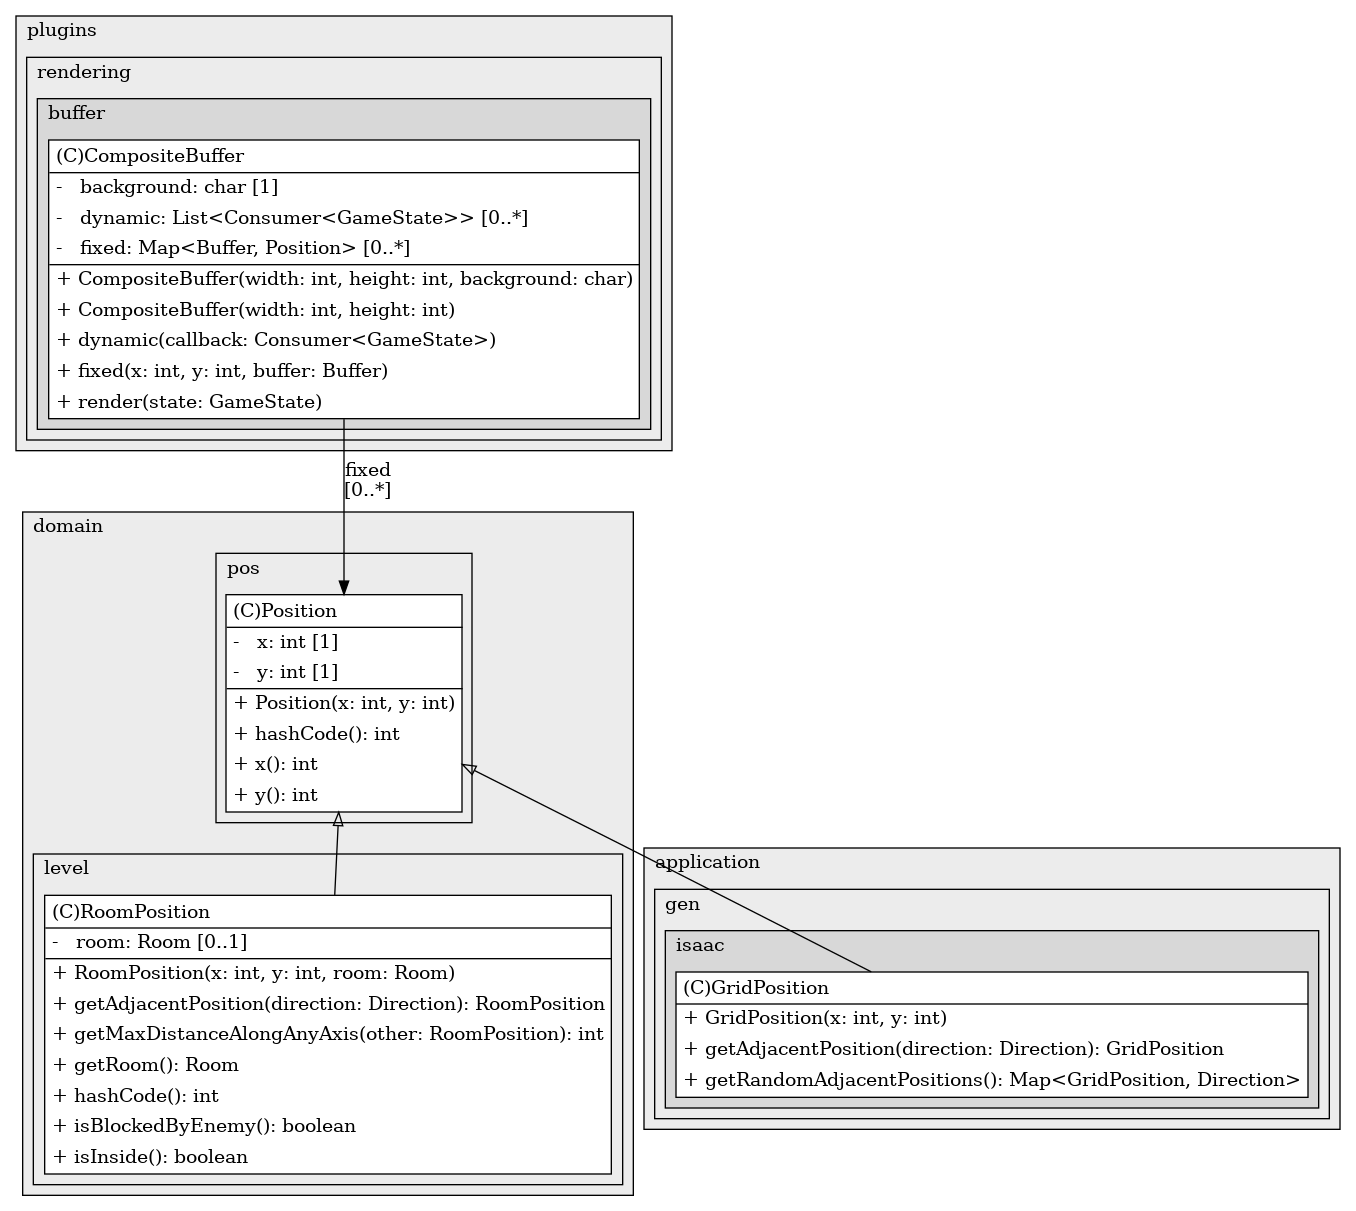
\includegraphics[width=0.9\linewidth]{Bilder/Visualisierung/Position_structure.png}
    \caption{Value Object \textit{Position}}
\end{figure}

\section{Repositories}
Die nachfolgende Abbildung zeigt das UML-Diagramm des Interface
\textit{IGameRepository}. Streng genommen sind mit \textit{Repositories}
Vermittlungsschichten zwischen der \textit{domain} und dem Datenmodell
gemeint. Hier ist es eine Vermittlung zwischen dem \textit{application}-
Layer und dem Persistenzspeicher. 

In diesem Fall ist das \textit{Repository} dazu gedacht, den gesamten
\textit{GameState} (Spielstand) auf einmal zu serialisieren und zu
speichern. Dieser ist jedoch Teil der \textit{application}-Schicht.
Statt jedoch alle Domönenkomponenten des \textit{GameState} einzeln
zu speichern und zu einem späteren Zeitpunkt wieder zu laden, ergibt
es Sinn die Definition zu lockern und stattdessen mit einem einzelnen
zentralen Objekt der \textit{application}- statt der \textit{Domänen}-
Schicht zu interagieren. Dies dient letztlich der Übersichtlichkeit
und Einfachheit.

Die Benutzung des \textit{IGameRepository} führt zu verringerter
Kopplung und erlaubt die Einhaltung der Dependency Rule und des OCP.
Es kann auf einfache Weise die Persistenzmethode ausgetauscht werden,
ohne dass andere Schichten von den Änderungen betroffen sind.

\vspace{0.5cm}
\begin{figure}[H]
    \centering
    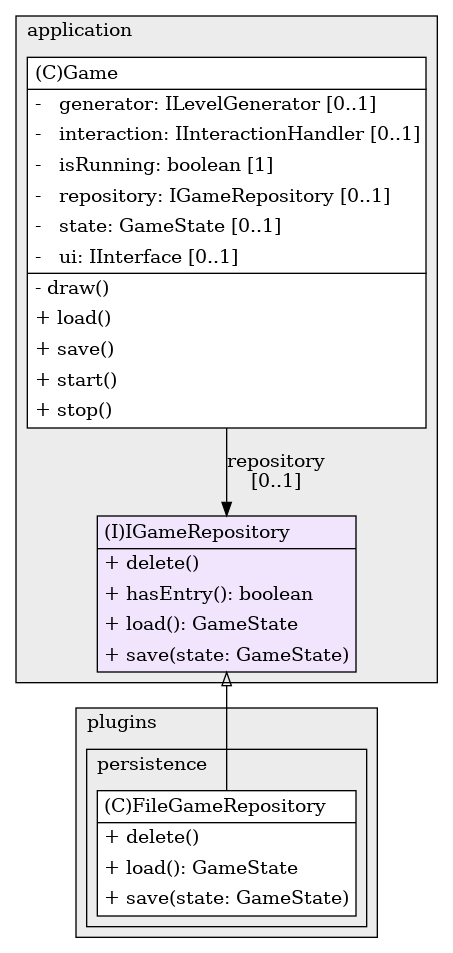
\includegraphics[width=0.3\linewidth]{Bilder/Visualisierung/IGameRepository_structure.png}
    \caption{Repositories \textit{IGameRepository}}
\end{figure}

\section{Aggregates}
Die nachfolgende Abbildung zeigt ein gekürztes UML-Diagramm zur Klasse
\textit{Room}, welche ein \textit{Aggregate} darstellt. Der \textit{Room}
stellt das Wurzel-Element der Verwaltungseinheit dar. Ihr zugeordnet
sind wichtige Eigenschaften, welche einen abgegrenzen Spielbereich
ausmachen. Dazu gehören Spielfeldmaße (\textit{width} und \textit{height}),
der \textit{Player}, Türen (\textit{Door}), \textit{Items} und Gegner
(\textit{Enemy}).

Das Aggregat ist genau wie seine Bestandteile in der \textit{domain}-
Schicht befindlich. Es sorgt für korrekte und konsistente Interaktion
mit seinen Bestandteilen. So gibt es etwa Verwaltungsfunktionen wie
\textit{addItem()} zum Hinzufügen von Items und \textit{removeItem()}
zum Entfernen. Jedes Element ist genau einem Raum zugeordnet. Es findet
keine Mehrfachverwaltung statt. Zudem reduziert es die Fehleranfälligkeit
und Komplexität durch Query-Funktionen wie \textit{getClosestEntity()},
welche enthaltene Informationen berechnet und weiterreicht. 

\vspace{0.5cm}
\begin{figure}[H]
    \centering
    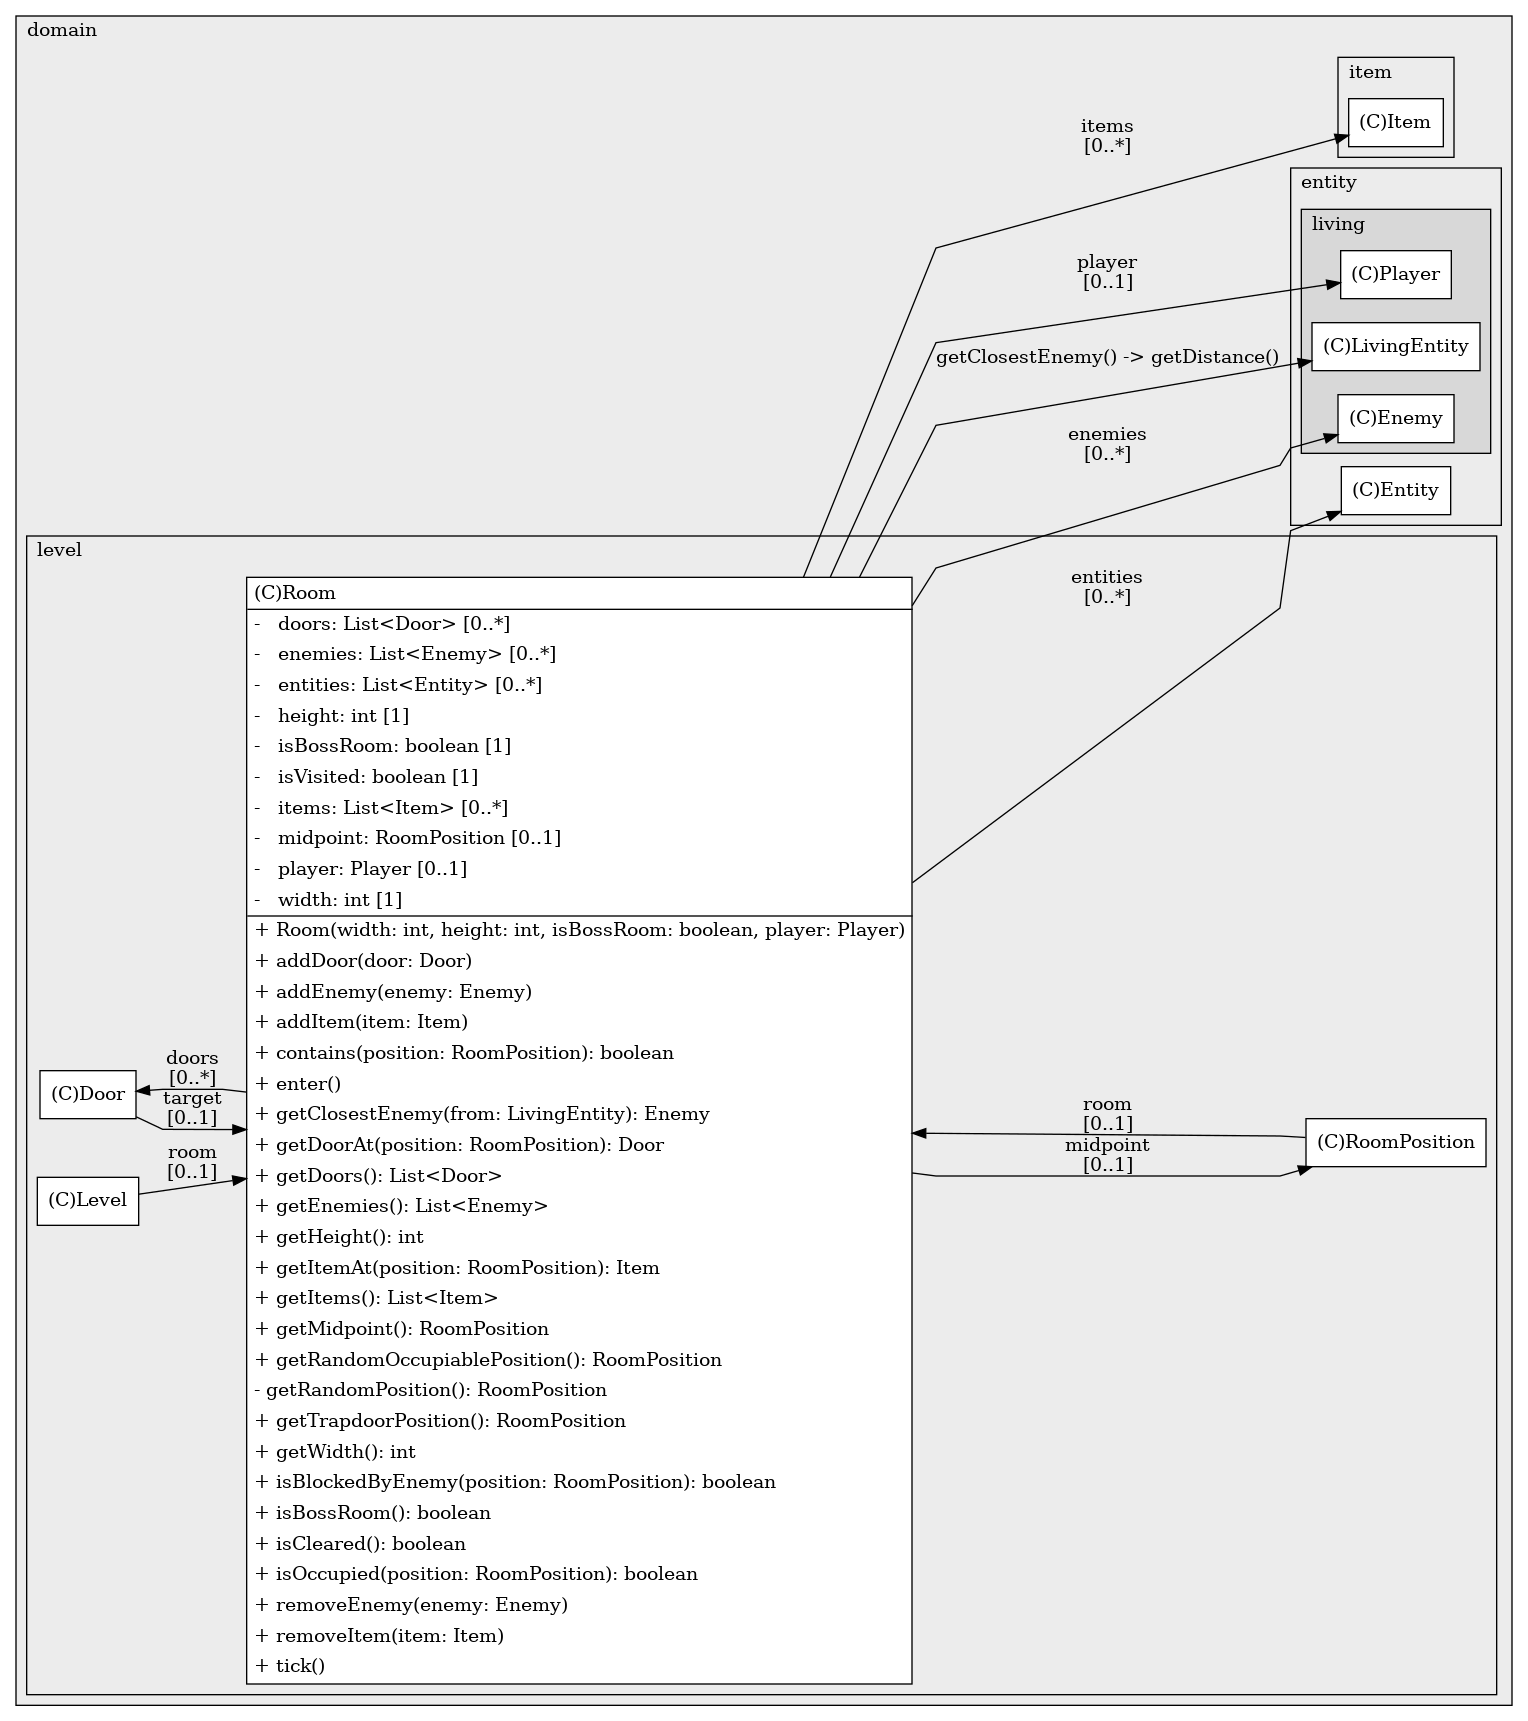
\includegraphics[width=1\linewidth]{Bilder/Visualisierung/RoomAggregate_structure.png}
    \caption{Aggregates \textit{Room}}
\end{figure}
